\chapter{Segmentation}
The goal of segmentation is to partition data into meaningful subsets. In heritage range images such groupings will often include, but are not limited to, points representing vegetation, walls, people or scanner artifacts. Isolating these points can be extremely difficult and time consuming. Suitable segmentation techniques should speed up the process by reducing a user's workload while maintaining interactivity.

% Interactive batch jobs

\section{Performance}
A key metric for measuring the performance of a technique is the time it takes for a user to achieve a segmentation result. The total segmentation time is the sum of durations associated with each user action. The time to perform a segmentation can thus be reduced by either minimizing the time consumed by individual actions or reducing the number of actions.

Reductions in the time consumed by an for manual actions can be achieved via a good user interface as discussed in discussed in \ref{chapter:framework}.The number of actions required by a user can be reduced by delegating work to an algorithm. It is important for an effective algorithm to produce a result within a reasonable amount of time. If a user could achieve an equivalent result without the algorithm in less time, the technique adds no value.

For non synthetic range images, it is unlikely that an algorithm will produce a perfect segmentation. It is thus expected that remedial action by a user will almost always be required. The final segmentation will thus be the sum of the time required for algorithm action and remedial user actions.

For example, if an automated tool for wall segmentation selected 95\% of the wall and part of a nearby tree, a complete segmentation will only be achieved once the remaining 5\% of the wall is selected and the tree points removed. If a user could previously perform the segmentation in 2 minutes, the automated tool would only be useful if it could allow a user complete the task in less than 2 minutes. If the wall segmentation tool needs 30 seconds to isolate the wall and then requires and additional 30 seconds of user action to refine the result, the tool can be considered useful as it can reduce the segmentation time by 1 minute. If however, the accuracy of the result is such that an additional 2 minutes of user action is required to achieve the same result, the tool provides no advantage over the status quo. The same can be said if the processing time pushed the total time over the 2 minute mark.

A high accuracy technique can minimize the amount of subsequent remedial user action required following its use. It should however be noted that accuracy is not directly related to reduced effort. Consider a wall selection tool that only selects 50\% of a target wall. If the missing points were clustered together and could be lasso selected with a single action, the total time could still be low. This wall selection tool would exhibit low accuracy but would still be extremely effective.


\section{Evaluation}

\begin{figure}[ht]
  \centering
  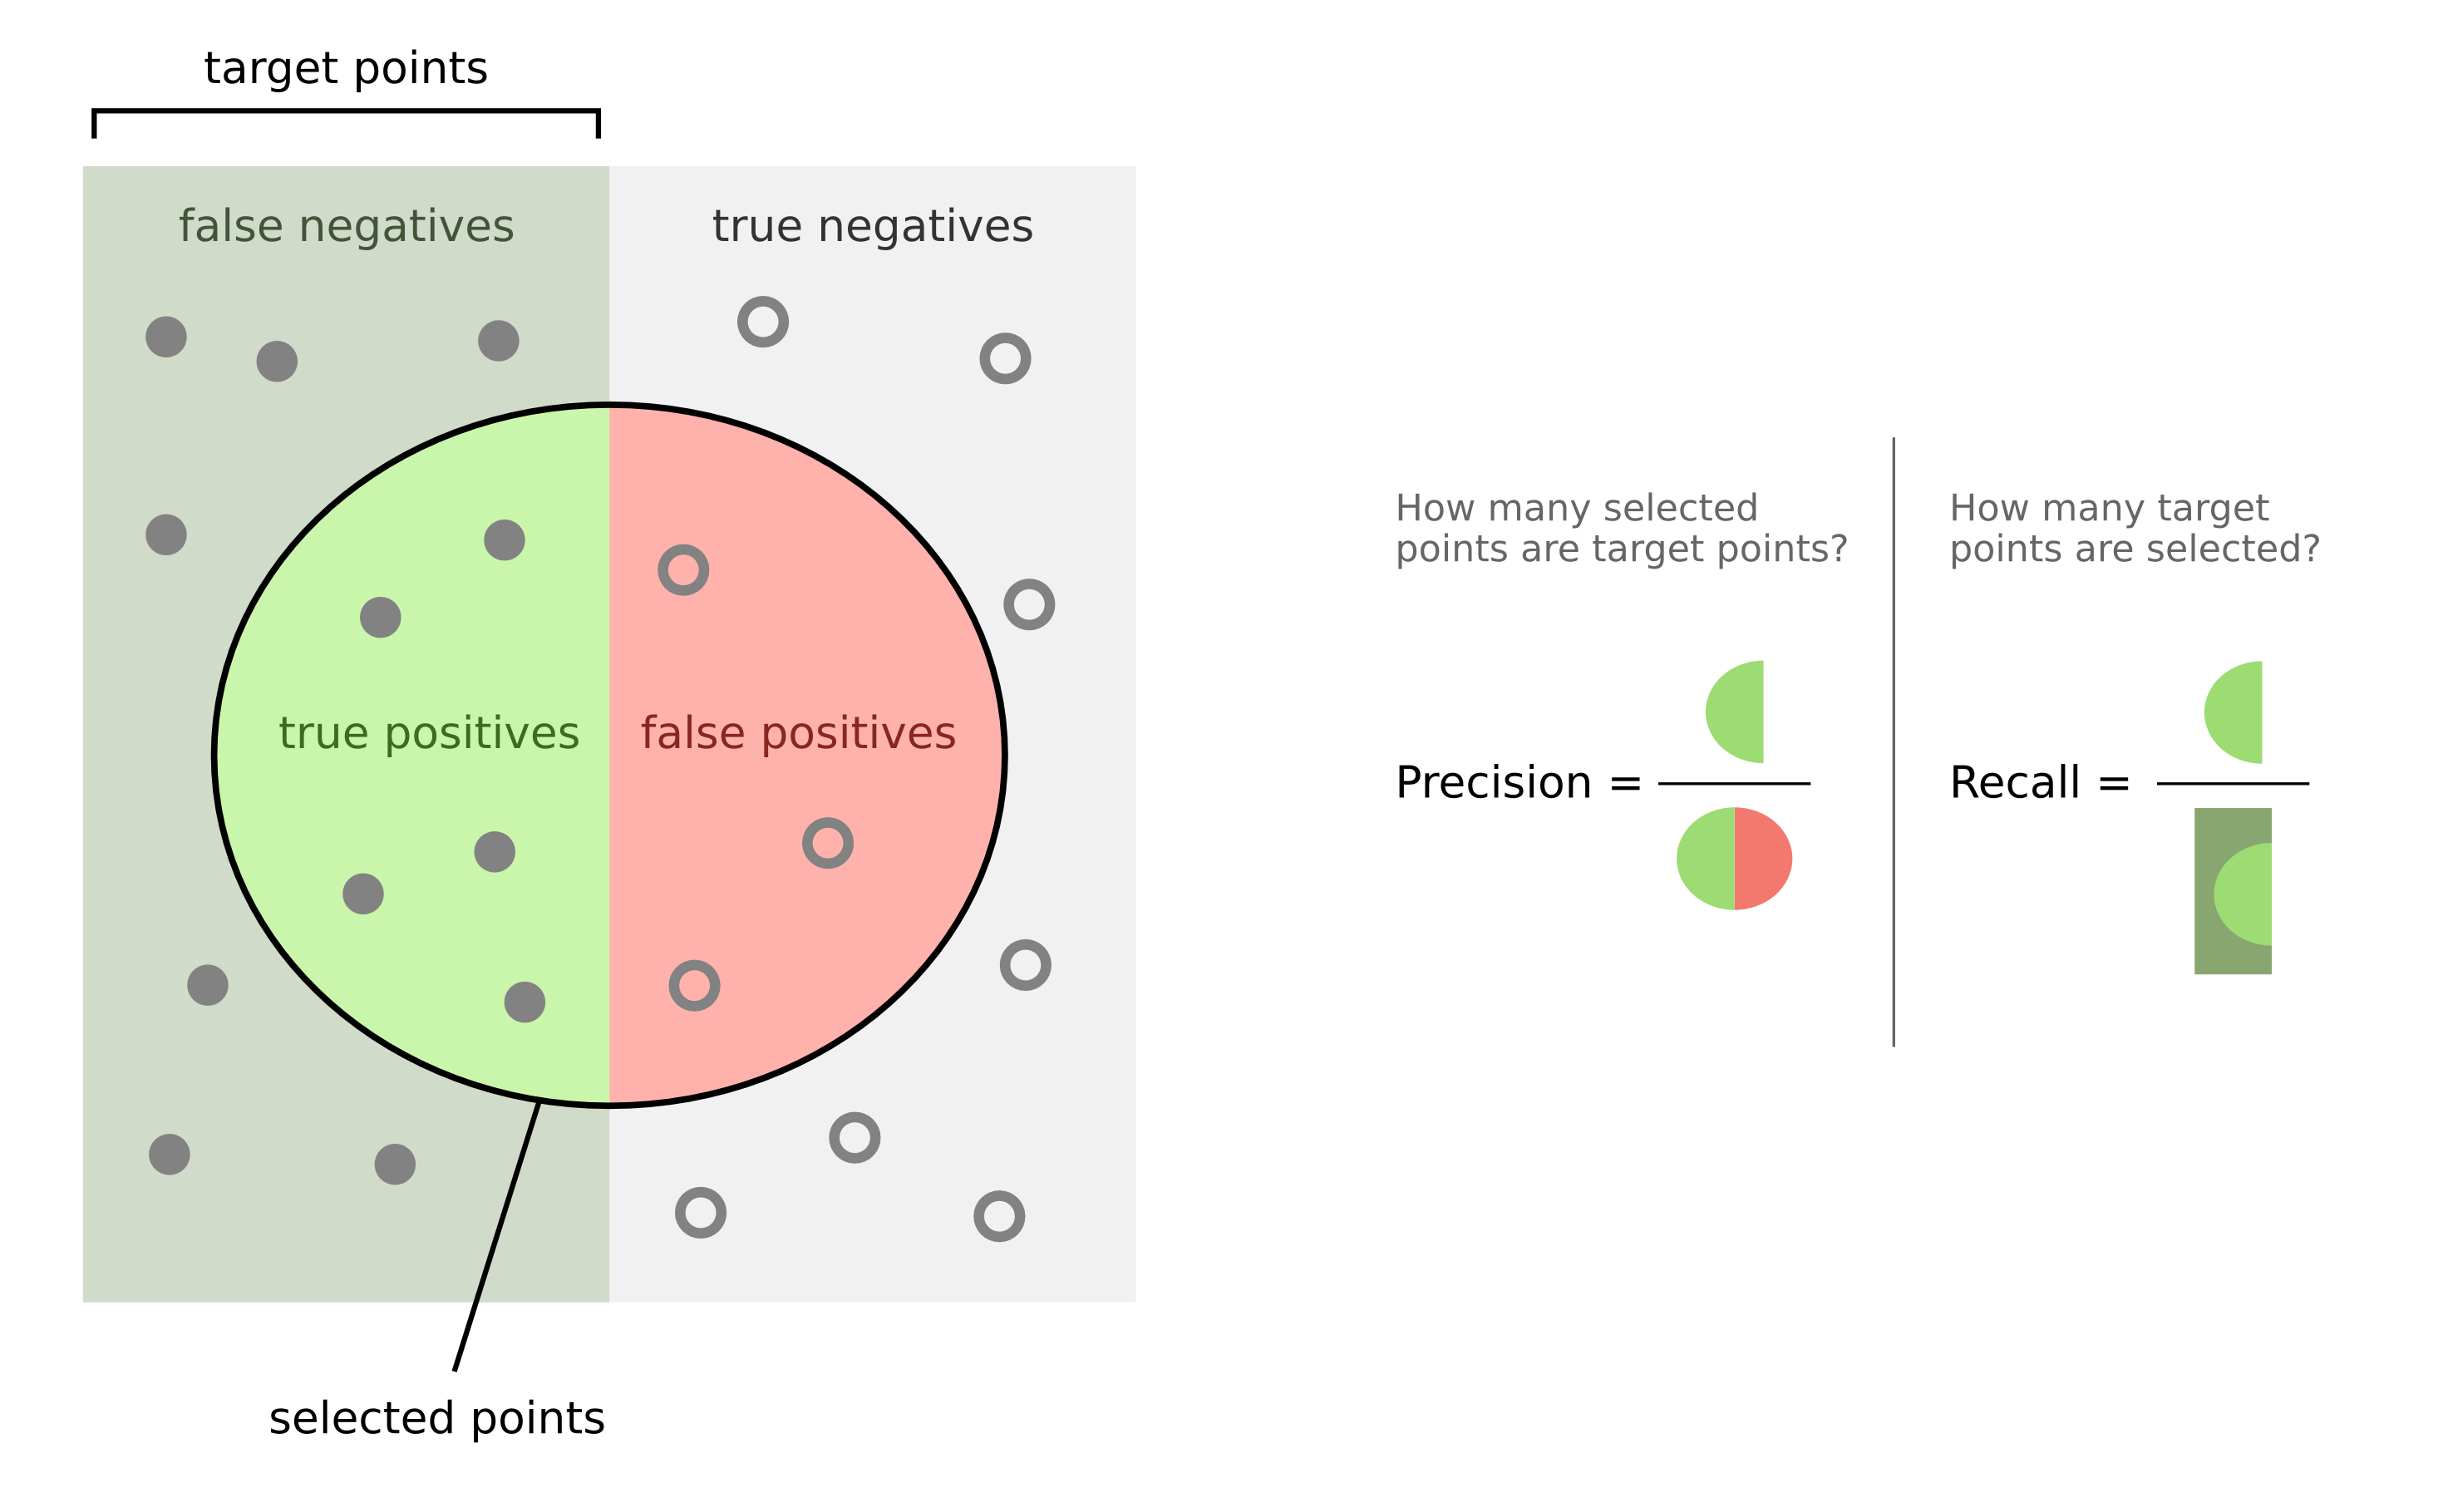
\includegraphics[width=1\linewidth]{images/precision_recall.png}
  \caption[Precision and recall]{Precision and recall protect\footnotemark[\value{footnote}] } 
  \label{fig:precision_recall}
\end{figure}
\footnotetext{Adapted from: \url{https://en.wikipedia.org/wiki/Precision_and_recall}}

Segmentation algorithms are typically evaluated in terms of precision and recall \cite{Ponce2012}. Given a set of points we define a subset as our target. If an algorithm selects another subset, the selected points can be divided into true positives and false negatives. The remaining points are either false negatives or true negatives (see \autoref{fig:precision_recall}).

Precision is then defined as the number of true positives selected as fraction of the total number of selected points.

\begin{equation} \label{eq:precision}
	\text{precision}=\frac{|\{\text{target points}\}\cap\{\text{selected points}\}|}{|\{\text{selected points}\}|}
   % \right.
\end{equation}

Recall is defined as the number of true positives as a fraction of the targeted points.

\begin{equation} \label{eq:recall}
	\text{recall}=\frac{|\{\text{target points}\}\cap\{\text{selected points}\}|}{|\{\text{selected points}\}|}
   % \right.
\end{equation}

These two measures can be combined as an F-score that represents accuracy. The score can be interpreted as the weighted average of precision and recall.

\begin{equation} \label{eq:f1score}
	F_1 = 2 \cdot \frac{\mathrm{precision} \cdot \mathrm{recall}}{\mathrm{precision} + \mathrm{recall}}
   % \right.
\end{equation}

Our position is unique in that user efficiency instead of accuracy is our primary objective. Accuracy is still a good indicator of how useful related research is likely to be. Computational efficiency however is at least as important as it contributes to the total task time.

% later present evaluation technique

\section{Segmentation methods}

Segmentation algorithms include a variety of related methods with the same goal of grouping related data points. Points can be grouped either by considering local or global relations. These two organizing principles are not always mutually exclusive. Techniques that group points via local relations are called called clustering methods. The goal is to ensure grouped points look like alike. As an example we may group together green points. The second set of techniques group points that share some global characteristic. Points that lie on a plane may be grouped because when seen as a whole the points represent a surface. These techniques are typically model driven.

\subsection{Features}

In order to group related points we need a way of comparing them. Intrinsic properties of the dataset such as 3D coordinates and intensity can be used. These properties are also called features. A feature vector is used to collect all relevant measurements that describe a point. We are not limited to intrinsic properties of a dataset. New features can be uncovered or created by processing a dataset. This process also known as feature extraction/engineering. A good feature will help achieve a segmentation result by bring forward similarities and dissimilarities between points. Features can also be used to summarize groups of points for further processing.


\subsection{Clustering methods}






% referred to as features and are organized into a feature vector.



% Grab cut

% forming image regions (sometimes use as the exclusive meaning of segmentation)
% 	decompose an image into regions that have roughly coherent color and texture.
% 	Typically, the shape of these regions isn’t particularly important, but the coherence is important
% 	regions allow us to deal with larger areas of an image without considering each element. (summary representation)
% 	super pixels can expose structure in images



% Clustering can be applied to points or groups of points

\subsection{Model driven methods}
% Model must account for variation, hard to define

% Hough transform
% Ransacs
% Machine learning


% Features
% 	What is a good feature
% 	How to design or pick a good feature?
% 		Something that correlates with what you are trying to segment?
% 		Only evaluated as part of a learning/segmentation/clustering algorithm?
% Clusters
% Interactive segmentation
% Machine learning
% 	Deep nets
% 		Learn features via unsupervised
% 	SVG
% 	Random forests
% 	Graph optimasation

% Existing systems
% 	Range images
% 	Point clouds
% 	Aerial scans
% 	What features are used?
% 	Clustering
% 	Machine learning
% 	Level of accuracy
% 	Interactive?
% 	Assumptions?

